% Options for packages loaded elsewhere
\PassOptionsToPackage{unicode}{hyperref}
\PassOptionsToPackage{hyphens}{url}
\PassOptionsToPackage{dvipsnames,svgnames,x11names}{xcolor}
%
\documentclass[
  letterpaper,
  DIV=11,
  numbers=noendperiod]{scrartcl}

\usepackage{amsmath,amssymb}
\usepackage{lmodern}
\usepackage{iftex}
\ifPDFTeX
  \usepackage[T1]{fontenc}
  \usepackage[utf8]{inputenc}
  \usepackage{textcomp} % provide euro and other symbols
\else % if luatex or xetex
  \usepackage{unicode-math}
  \defaultfontfeatures{Scale=MatchLowercase}
  \defaultfontfeatures[\rmfamily]{Ligatures=TeX,Scale=1}
\fi
% Use upquote if available, for straight quotes in verbatim environments
\IfFileExists{upquote.sty}{\usepackage{upquote}}{}
\IfFileExists{microtype.sty}{% use microtype if available
  \usepackage[]{microtype}
  \UseMicrotypeSet[protrusion]{basicmath} % disable protrusion for tt fonts
}{}
\makeatletter
\@ifundefined{KOMAClassName}{% if non-KOMA class
  \IfFileExists{parskip.sty}{%
    \usepackage{parskip}
  }{% else
    \setlength{\parindent}{0pt}
    \setlength{\parskip}{6pt plus 2pt minus 1pt}}
}{% if KOMA class
  \KOMAoptions{parskip=half}}
\makeatother
\usepackage{xcolor}
\usepackage[normalem]{ulem}
\setlength{\emergencystretch}{3em} % prevent overfull lines
\setcounter{secnumdepth}{-\maxdimen} % remove section numbering
% Make \paragraph and \subparagraph free-standing
\ifx\paragraph\undefined\else
  \let\oldparagraph\paragraph
  \renewcommand{\paragraph}[1]{\oldparagraph{#1}\mbox{}}
\fi
\ifx\subparagraph\undefined\else
  \let\oldsubparagraph\subparagraph
  \renewcommand{\subparagraph}[1]{\oldsubparagraph{#1}\mbox{}}
\fi

\usepackage{color}
\usepackage{fancyvrb}
\newcommand{\VerbBar}{|}
\newcommand{\VERB}{\Verb[commandchars=\\\{\}]}
\DefineVerbatimEnvironment{Highlighting}{Verbatim}{commandchars=\\\{\}}
% Add ',fontsize=\small' for more characters per line
\usepackage{framed}
\definecolor{shadecolor}{RGB}{241,243,245}
\newenvironment{Shaded}{\begin{snugshade}}{\end{snugshade}}
\newcommand{\AlertTok}[1]{\textcolor[rgb]{0.68,0.00,0.00}{#1}}
\newcommand{\AnnotationTok}[1]{\textcolor[rgb]{0.37,0.37,0.37}{#1}}
\newcommand{\AttributeTok}[1]{\textcolor[rgb]{0.40,0.45,0.13}{#1}}
\newcommand{\BaseNTok}[1]{\textcolor[rgb]{0.68,0.00,0.00}{#1}}
\newcommand{\BuiltInTok}[1]{\textcolor[rgb]{0.00,0.23,0.31}{#1}}
\newcommand{\CharTok}[1]{\textcolor[rgb]{0.13,0.47,0.30}{#1}}
\newcommand{\CommentTok}[1]{\textcolor[rgb]{0.37,0.37,0.37}{#1}}
\newcommand{\CommentVarTok}[1]{\textcolor[rgb]{0.37,0.37,0.37}{\textit{#1}}}
\newcommand{\ConstantTok}[1]{\textcolor[rgb]{0.56,0.35,0.01}{#1}}
\newcommand{\ControlFlowTok}[1]{\textcolor[rgb]{0.00,0.23,0.31}{#1}}
\newcommand{\DataTypeTok}[1]{\textcolor[rgb]{0.68,0.00,0.00}{#1}}
\newcommand{\DecValTok}[1]{\textcolor[rgb]{0.68,0.00,0.00}{#1}}
\newcommand{\DocumentationTok}[1]{\textcolor[rgb]{0.37,0.37,0.37}{\textit{#1}}}
\newcommand{\ErrorTok}[1]{\textcolor[rgb]{0.68,0.00,0.00}{#1}}
\newcommand{\ExtensionTok}[1]{\textcolor[rgb]{0.00,0.23,0.31}{#1}}
\newcommand{\FloatTok}[1]{\textcolor[rgb]{0.68,0.00,0.00}{#1}}
\newcommand{\FunctionTok}[1]{\textcolor[rgb]{0.28,0.35,0.67}{#1}}
\newcommand{\ImportTok}[1]{\textcolor[rgb]{0.00,0.46,0.62}{#1}}
\newcommand{\InformationTok}[1]{\textcolor[rgb]{0.37,0.37,0.37}{#1}}
\newcommand{\KeywordTok}[1]{\textcolor[rgb]{0.00,0.23,0.31}{#1}}
\newcommand{\NormalTok}[1]{\textcolor[rgb]{0.00,0.23,0.31}{#1}}
\newcommand{\OperatorTok}[1]{\textcolor[rgb]{0.37,0.37,0.37}{#1}}
\newcommand{\OtherTok}[1]{\textcolor[rgb]{0.00,0.23,0.31}{#1}}
\newcommand{\PreprocessorTok}[1]{\textcolor[rgb]{0.68,0.00,0.00}{#1}}
\newcommand{\RegionMarkerTok}[1]{\textcolor[rgb]{0.00,0.23,0.31}{#1}}
\newcommand{\SpecialCharTok}[1]{\textcolor[rgb]{0.37,0.37,0.37}{#1}}
\newcommand{\SpecialStringTok}[1]{\textcolor[rgb]{0.13,0.47,0.30}{#1}}
\newcommand{\StringTok}[1]{\textcolor[rgb]{0.13,0.47,0.30}{#1}}
\newcommand{\VariableTok}[1]{\textcolor[rgb]{0.07,0.07,0.07}{#1}}
\newcommand{\VerbatimStringTok}[1]{\textcolor[rgb]{0.13,0.47,0.30}{#1}}
\newcommand{\WarningTok}[1]{\textcolor[rgb]{0.37,0.37,0.37}{\textit{#1}}}

\providecommand{\tightlist}{%
  \setlength{\itemsep}{0pt}\setlength{\parskip}{0pt}}\usepackage{longtable,booktabs,array}
\usepackage{calc} % for calculating minipage widths
% Correct order of tables after \paragraph or \subparagraph
\usepackage{etoolbox}
\makeatletter
\patchcmd\longtable{\par}{\if@noskipsec\mbox{}\fi\par}{}{}
\makeatother
% Allow footnotes in longtable head/foot
\IfFileExists{footnotehyper.sty}{\usepackage{footnotehyper}}{\usepackage{footnote}}
\makesavenoteenv{longtable}
\usepackage{graphicx}
\makeatletter
\def\maxwidth{\ifdim\Gin@nat@width>\linewidth\linewidth\else\Gin@nat@width\fi}
\def\maxheight{\ifdim\Gin@nat@height>\textheight\textheight\else\Gin@nat@height\fi}
\makeatother
% Scale images if necessary, so that they will not overflow the page
% margins by default, and it is still possible to overwrite the defaults
% using explicit options in \includegraphics[width, height, ...]{}
\setkeys{Gin}{width=\maxwidth,height=\maxheight,keepaspectratio}
% Set default figure placement to htbp
\makeatletter
\def\fps@figure{htbp}
\makeatother

\KOMAoption{captions}{tableheading}
\makeatletter
\@ifpackageloaded{tcolorbox}{}{\usepackage[many]{tcolorbox}}
\@ifpackageloaded{fontawesome5}{}{\usepackage{fontawesome5}}
\definecolor{quarto-callout-color}{HTML}{909090}
\definecolor{quarto-callout-note-color}{HTML}{0758E5}
\definecolor{quarto-callout-important-color}{HTML}{CC1914}
\definecolor{quarto-callout-warning-color}{HTML}{EB9113}
\definecolor{quarto-callout-tip-color}{HTML}{00A047}
\definecolor{quarto-callout-caution-color}{HTML}{FC5300}
\definecolor{quarto-callout-color-frame}{HTML}{acacac}
\definecolor{quarto-callout-note-color-frame}{HTML}{4582ec}
\definecolor{quarto-callout-important-color-frame}{HTML}{d9534f}
\definecolor{quarto-callout-warning-color-frame}{HTML}{f0ad4e}
\definecolor{quarto-callout-tip-color-frame}{HTML}{02b875}
\definecolor{quarto-callout-caution-color-frame}{HTML}{fd7e14}
\makeatother
\makeatletter
\makeatother
\makeatletter
\makeatother
\makeatletter
\@ifpackageloaded{caption}{}{\usepackage{caption}}
\AtBeginDocument{%
\ifdefined\contentsname
  \renewcommand*\contentsname{Table of contents}
\else
  \newcommand\contentsname{Table of contents}
\fi
\ifdefined\listfigurename
  \renewcommand*\listfigurename{List of Figures}
\else
  \newcommand\listfigurename{List of Figures}
\fi
\ifdefined\listtablename
  \renewcommand*\listtablename{List of Tables}
\else
  \newcommand\listtablename{List of Tables}
\fi
\ifdefined\figurename
  \renewcommand*\figurename{Figure}
\else
  \newcommand\figurename{Figure}
\fi
\ifdefined\tablename
  \renewcommand*\tablename{Table}
\else
  \newcommand\tablename{Table}
\fi
}
\@ifpackageloaded{float}{}{\usepackage{float}}
\floatstyle{ruled}
\@ifundefined{c@chapter}{\newfloat{codelisting}{h}{lop}}{\newfloat{codelisting}{h}{lop}[chapter]}
\floatname{codelisting}{Listing}
\newcommand*\listoflistings{\listof{codelisting}{List of Listings}}
\makeatother
\makeatletter
\@ifpackageloaded{caption}{}{\usepackage{caption}}
\@ifpackageloaded{subcaption}{}{\usepackage{subcaption}}
\makeatother
\makeatletter
\@ifpackageloaded{tcolorbox}{}{\usepackage[many]{tcolorbox}}
\makeatother
\makeatletter
\@ifundefined{shadecolor}{\definecolor{shadecolor}{rgb}{.97, .97, .97}}
\makeatother
\makeatletter
\makeatother
\ifLuaTeX
  \usepackage{selnolig}  % disable illegal ligatures
\fi
\IfFileExists{bookmark.sty}{\usepackage{bookmark}}{\usepackage{hyperref}}
\IfFileExists{xurl.sty}{\usepackage{xurl}}{} % add URL line breaks if available
\urlstyle{same} % disable monospaced font for URLs
\hypersetup{
  pdftitle={Introduction to Quarto},
  pdfauthor={Mattias Villani},
  colorlinks=true,
  linkcolor={blue},
  filecolor={Maroon},
  citecolor={Blue},
  urlcolor={Blue},
  pdfcreator={LaTeX via pandoc}}

\title{Introduction to Quarto}
\author{Mattias Villani}
\date{}

\begin{document}
\maketitle
\ifdefined\Shaded\renewenvironment{Shaded}{\begin{tcolorbox}[borderline west={3pt}{0pt}{shadecolor}, interior hidden, boxrule=0pt, sharp corners, enhanced, frame hidden, breakable]}{\end{tcolorbox}}\fi

\hypertarget{introduction}{%
\subsection{1. Introduction}\label{introduction}}

Quarto is a way to integrate text (markdown), computer code, figures,
tables and mathematical formulas in one document.\\
Quarto documents (with file ending .qmd) can easily be turned into pdf
format, html, website, blogs and presentations.

\hypertarget{settings-for-the-document---the-yaml}{%
\subsection{2. Settings for the document - the
YAML}\label{settings-for-the-document---the-yaml}}

At the top of a quarto document is the so called YAML, which tells the
Quarto engine how the document should be formatted. This is the YAML for
this document:

\begin{figure}

{\centering 
\includegraphics{yaml.png}

}

\end{figure}

which basically only gives the title and author information, everything
else is using default settings. This will print (\textbf{render}) the
document to html by default. If I instead wanted to render to pdf I
would use the YAML:

\begin{figure}

{\centering 
\includegraphics{yaml_pdf.png}

}

\end{figure}

\hypertarget{writing-formatted-text-using-markdown}{%
\subsection{3. Writing formatted text using
markdown}\label{writing-formatted-text-using-markdown}}

The text written in a Quarto document can be formatted using the
\textbf{markdown} language. Markdown is a very simple language for
formatting text. For example, I can easily make the text \textbf{bold}
by writing \texttt{**bold**} or \emph{italic} using a single * on each
side of the text. A bulleted list:

\begin{itemize}
\item
  bullet
\item
  list
\item
  are also
\item
  easy
\end{itemize}

is produced by putting a dash \texttt{-} and space before each bullet
point. Numbered lists are also simple, just place numbers and a dot (.)
before each list item. Like this:

\begin{enumerate}
\def\labelenumi{\arabic{enumi}.}
\tightlist
\item
  This is the first point
\item
  and this is second
\item
  and so on.
\end{enumerate}

Images can be inserted by typing
\texttt{!{[}sceptic\ larry{]}(/misc/larry.png)\{width="100"\}} which
would give the picture below. So the text caption for the image is
written between the brackets {[}{]} and the search path to the image on
your computer is given inside the parentheses ().

\begin{figure}

{\centering 
\includegraphics[width=1.04167in,height=\textheight]{../../misc/larry.png}

}

\caption{sceptic larry}

\end{figure}

You can leave out the figure text and the width argument and just write:
\texttt{!{[}{]}(/misc/larry.png)} .

Tables are also pretty easy. The table below is made by writing

\texttt{\textbar{}\ Name\ \ \textbar{}\ Age\ \textbar{}\ Position\ \ \ \ \ \ \ \ \ \ \ \ \textbar{}}

\texttt{\textbar{}-\/-\/-\/-\/-\/-\/-\textbar{}-\/-\/-\/-\/-\textbar{}-\/-\/-\/-\/-\/-\/-\/-\/-\/-\/-\/-\/-\/-\/-\/-\/-\/-\/-\/-\/-\textbar{}}

\texttt{\textbar{}\ Mike\ \ \textbar{}\ 49\ \ \textbar{}\ Professor\ \ \ \ \ \ \ \ \ \ \ \textbar{}}

\texttt{\textbar{}\ Sarah\ \textbar{}\ 37\ \ \textbar{}\ Assistant\ professor\ \textbar{}}

\texttt{\textbar{}\ Anne\ \ \textbar{}\ 26\ \ \textbar{}\ PhD\ student\ \ \ \ \ \ \ \ \ \textbar{}}

\begin{longtable}[]{@{}lll@{}}
\caption{A little table caption.}\tabularnewline
\toprule()
Name & Age & Position \\
\midrule()
\endfirsthead
\toprule()
Name & Age & Position \\
\midrule()
\endhead
Mike & 49 & Professor \\
Sarah & 37 & Assistant professor \\
Anne & 26 & PhD student \\
\bottomrule()
\end{longtable}

What if you want the table caption text to be below the tables, not
below it? No sweat, just put \texttt{table-cap-location:\ bottom} in
your YAML at the top of the document.

\hypertarget{writing-code}{%
\subsection{4. Writing code}\label{writing-code}}

A Quarto document can have executable code in them. It supports several
programming languages, most notably: R, Python and Julia. You just need
to add a \textbf{code chunk}. A code chunk starts and ends with three so
called backticks `. The backtick is typed by \texttt{Shift} and the key
to the left of \texttt{Backspace} on a Swedish keyboard. This is a chunk
of R code:

\begin{figure}

{\centering 
\includegraphics{codechunk.png}

}

\end{figure}

Note the little green Play-button. By pressing that we can run the code
chunk. After running the code in the Quarto-document, the variables (in
this case a vector \texttt{x}) will be available in the console, just
like for any R code. Here is the end result of that code chunk:

\begin{Shaded}
\begin{Highlighting}[]
\NormalTok{x }\OtherTok{=} \FunctionTok{rnorm}\NormalTok{(}\DecValTok{100}\NormalTok{)}
\FunctionTok{plot}\NormalTok{(x, }\AttributeTok{type =} \StringTok{"l"}\NormalTok{, }\AttributeTok{xlab =} \StringTok{"time"}\NormalTok{, }\AttributeTok{main =} \StringTok{"time series plot"}\NormalTok{)}
\end{Highlighting}
\end{Shaded}

\begin{figure}[H]

{\centering 
\includegraphics{Intro2Quarto_files/figure-pdf/unnamed-chunk-1-1.pdf}

}

\end{figure}

\begin{tcolorbox}[enhanced jigsaw, left=2mm, opacityback=0, colframe=quarto-callout-tip-color-frame, breakable, colback=white, bottomrule=.15mm, arc=.35mm, leftrule=.75mm, rightrule=.15mm, toprule=.15mm]
\begin{minipage}[t]{5.5mm}
\textcolor{quarto-callout-tip-color}{\faLightbulb}
\end{minipage}%
\begin{minipage}[t]{\textwidth - 5.5mm}
Quarto supports other popular programming languages in addtion to

\includegraphics[width=0.20833in,height=\textheight]{/misc/R.jpeg}.

A chunk of Python

\includegraphics[width=0.20833in,height=\textheight]{/misc/python.png}
code would start with
\texttt{\textasciigrave{}\textasciigrave{}\textasciigrave{}\{python\}}.

A Julia

\includegraphics[width=0.20833in,height=0.19792in]{/misc/julia.png} code
chunk starts with
\texttt{\textasciigrave{}\textasciigrave{}\textasciigrave{}\{julia\}}.

\includegraphics[width=0.20833in,height=\textheight]{/misc/hearteyes.png}\end{minipage}%
\end{tcolorbox}

What if I want to use the code to produce the plot, but not show the
code in my report? Easy, I would just add some YAML information at the
beginning of the code chunk itself. YAML inside of a code chunk must
begin with the two characters \texttt{\#\textbar{}} . Here is how you
hide the code:

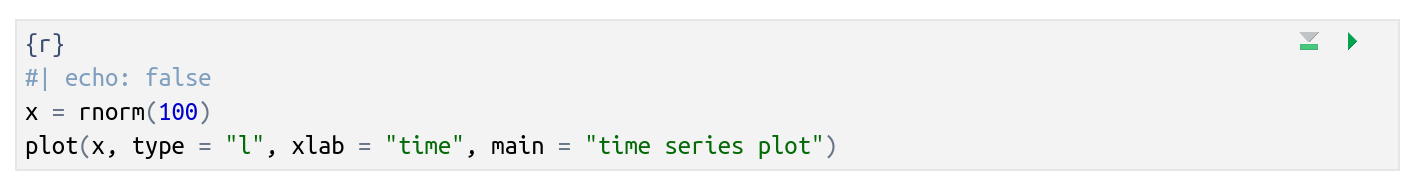
\includegraphics{codechunkechofalse.png}

The first character \texttt{\#} is called a \textbf{hash} and the second
\texttt{\textbar{}} a \textbf{pipe}. So the recommended way to remember
\texttt{\#\textbar{}} is by thinking of the Weezer song:
\href{https://www.youtube.com/watch?v=fg_68MBzpzQ\&ab_channel=Weezer-Topic}{hash
pipe}. BTW, there I used a \textbf{hyperlink} which you write as
\texttt{{[}link\ text{]}(webpage\ address)} where the webpage address is
a http-link, but can also be links within a document.

\hypertarget{writing-mathematical-formulas}{%
\subsection{5. Writing mathematical
formulas}\label{writing-mathematical-formulas}}

Quarto supports LaTeX, which is a professional typesetting system for
mathematical symbols. LaTeX takes a while to master, but you can look it
up online to learn the basics. Just enclose LaTeX code between two
dollar-signs on each side. Here is a simple example
\texttt{\$\$\textbackslash{}alpha\_1\$\$} which would come out as
\[\alpha_1\] in your document. Here is a more complex example:

\texttt{\$\$\textbackslash{}bar\{x\}\ =\ \textbackslash{}frac\{1\}\{n\}\textbackslash{}sum\_\{i=1\}\^{}n\ x\_i\$\$}

which would come out as the formula for the sample mean:

\[\bar{x} = \frac{1}{n}\sum_{i=1}^n x_i\]

\hypertarget{using-the-visual-editor-in-rstudio}{%
\subsection{6. Using the Visual editor in
RStudio}\label{using-the-visual-editor-in-rstudio}}

You can create (\uline{\textbf{F}}\textbf{ile}/\textbf{New
\uline{F}ile}/\uline{\textbf{Q}}\textbf{uarto document\ldots{}} menu)
and write Quarto documents in RStudio. When you open a Quarto document
in the editor the menu bar changes to (may look different for you):

\begin{figure}

{\centering 
\includegraphics{quarto_menu_bar.png}

}

\end{figure}

Clicking on the \texttt{Render} button will render the document to html
(default) or pdf (if you choose that in the YAML). Pressing the
\texttt{Run} button will re-run all the code chunks in the document. You
can write your Quarto document as markdown code if you click the
\texttt{Source} -button in the extreme left. If you press the
\texttt{Visual}-button you will see the document in a similar way to
word processors like Word. You can then insert images and table, change
font sizes etc by clicking on the menu. I tend to spend most time in
Visual mode, but will often go over to Source mode when I want absolute
control of what I do.

\hypertarget{going-fancy---interactivity}{%
\subsection{7. Going fancy -
interactivity}\label{going-fancy---interactivity}}

Quarto documents have the basic interactivity that one can change code
inside a code chunk, render the document and everything in the document
changes according to the changes in the code.

\hfill\break
But it also possible to make the final html interactive. Below is an an
example to wet your appetite. Note however that you need to view the
html file in an external web browser and not using the Viewer inside
RStudio. Try moving around the slides to change the plot.

\begin{Shaded}
\begin{Highlighting}[]
\NormalTok{//| echo: false}
\NormalTok{data = FileAttachment("palmer{-}penguins.csv").csv(\{ typed: true \})}
\end{Highlighting}
\end{Shaded}

\begin{Shaded}
\begin{Highlighting}[]
\NormalTok{//| echo: false}
\NormalTok{viewof bill\_length\_min = Inputs.range(}
\NormalTok{  [32, 50], }
\NormalTok{  \{value: 35, step: 1, label: "Bill length (min):"\}}
\NormalTok{)}
\NormalTok{viewof islands = Inputs.checkbox(}
\NormalTok{  ["Torgersen", "Biscoe", "Dream"], }
\NormalTok{  \{ value: ["Torgersen", "Biscoe"], }
\NormalTok{    label: "Islands:"}
\NormalTok{  \}}
\NormalTok{)}
\end{Highlighting}
\end{Shaded}

\begin{Shaded}
\begin{Highlighting}[]
\NormalTok{//| echo: false}
\NormalTok{filtered = data.filter(function(penguin) \{}
\NormalTok{  return bill\_length\_min \textless{} penguin.bill\_length\_mm \&\&}
\NormalTok{         islands.includes(penguin.island);}
\NormalTok{\})}
\end{Highlighting}
\end{Shaded}

\hypertarget{plot}{%
\paragraph{Plot}\label{plot}}

\begin{Shaded}
\begin{Highlighting}[]
\NormalTok{//| echo: false}
\NormalTok{Plot.rectY(filtered, }
\NormalTok{  Plot.binX(}
\NormalTok{    \{y: "count"\}, }
\NormalTok{    \{x: "body\_mass\_g", fill: "species", thresholds: 20\}}
\NormalTok{  ))}
\NormalTok{  .plot(\{}
\NormalTok{    facet: \{}
\NormalTok{      data: filtered,}
\NormalTok{      x: "sex",}
\NormalTok{      y: "species",}
\NormalTok{      marginRight: 80}
\NormalTok{    \},}
\NormalTok{    marks: [}
\NormalTok{      Plot.frame(),}
\NormalTok{    ]}
\NormalTok{  \}}
\NormalTok{)}
\end{Highlighting}
\end{Shaded}

\hypertarget{data}{%
\paragraph{Data}\label{data}}

\begin{Shaded}
\begin{Highlighting}[]
\NormalTok{//| echo: false}
\NormalTok{Inputs.table(filtered)}
\end{Highlighting}
\end{Shaded}




\end{document}
